%%%%%%%%%%%%%%%%%%%%%%%%%%%%%%%%%%%%%%%%%%%%%%%%%%%%%%%%%%%%%%%%%%%%%%%%%%%
%  hw1.Rnw
%   
%  Autor: Alexandro Mayoral <https://github.com/bluepill5>  
% 
%%%%%%%%%%%%%%%%%%%%%%%%%%%%%%%%%%%%%%%%%%%%%%%%%%%%%%%%%%%%%%%%%%%%%%%%%%

\documentclass[a4paper]{scrartcl}\usepackage[]{graphicx}\usepackage[]{color}
%% maxwidth is the original width if it is less than linewidth
%% otherwise use linewidth (to make sure the graphics do not exceed the margin)
\makeatletter
\def\maxwidth{ %
  \ifdim\Gin@nat@width>\linewidth
    \linewidth
  \else
    \Gin@nat@width
  \fi
}
\makeatother

\definecolor{fgcolor}{rgb}{0.345, 0.345, 0.345}
\newcommand{\hlnum}[1]{\textcolor[rgb]{0.686,0.059,0.569}{#1}}%
\newcommand{\hlstr}[1]{\textcolor[rgb]{0.192,0.494,0.8}{#1}}%
\newcommand{\hlcom}[1]{\textcolor[rgb]{0.678,0.584,0.686}{\textit{#1}}}%
\newcommand{\hlopt}[1]{\textcolor[rgb]{0,0,0}{#1}}%
\newcommand{\hlstd}[1]{\textcolor[rgb]{0.345,0.345,0.345}{#1}}%
\newcommand{\hlkwa}[1]{\textcolor[rgb]{0.161,0.373,0.58}{\textbf{#1}}}%
\newcommand{\hlkwb}[1]{\textcolor[rgb]{0.69,0.353,0.396}{#1}}%
\newcommand{\hlkwc}[1]{\textcolor[rgb]{0.333,0.667,0.333}{#1}}%
\newcommand{\hlkwd}[1]{\textcolor[rgb]{0.737,0.353,0.396}{\textbf{#1}}}%

\usepackage{framed}
\makeatletter
\newenvironment{kframe}{%
 \def\at@end@of@kframe{}%
 \ifinner\ifhmode%
  \def\at@end@of@kframe{\end{minipage}}%
  \begin{minipage}{\columnwidth}%
 \fi\fi%
 \def\FrameCommand##1{\hskip\@totalleftmargin \hskip-\fboxsep
 \colorbox{shadecolor}{##1}\hskip-\fboxsep
     % There is no \\@totalrightmargin, so:
     \hskip-\linewidth \hskip-\@totalleftmargin \hskip\columnwidth}%
 \MakeFramed {\advance\hsize-\width
   \@totalleftmargin\z@ \linewidth\hsize
   \@setminipage}}%
 {\par\unskip\endMakeFramed%
 \at@end@of@kframe}
\makeatother

\definecolor{shadecolor}{rgb}{.97, .97, .97}
\definecolor{messagecolor}{rgb}{0, 0, 0}
\definecolor{warningcolor}{rgb}{1, 0, 1}
\definecolor{errorcolor}{rgb}{1, 0, 0}
\newenvironment{knitrout}{}{} % an empty environment to be redefined in TeX

\usepackage{alltt}

% Librerías necesarias
\usepackage[utf8]{inputenc}
\usepackage{amsmath}
\usepackage{amsfonts}
\usepackage{amssymb}
\usepackage{enumerate}
\usepackage{fullpage} % Maximiza el uso del espacio en la hoja.
\usepackage[left=2cm,right=2cm,top=2cm,bottom=2cm]{geometry}
\usepackage{dcolumn}
\usepackage{rotating}
\usepackage{float}
\usepackage[section]{placeins}
\usepackage{needspace}
\usepackage{hyperref}
\usepackage{setspace}
\usepackage{pifont}
\usepackage{adjustbox}
\usepackage[table,xcdraw]{xcolor}
\usepackage{graphics}
\onehalfspacing

\author{Alexandro Mayoral, Daniela Chávez y Gerardo Vazquez}
\title{Tarea 1 Análisis y Diseño de Experimentos}
\date{15/04/2015}
\IfFileExists{upquote.sty}{\usepackage{upquote}}{}
\begin{document}
\maketitle




\textbf{Problema 1}
Considere una variable aleatoria $X \sim N(0.5, 1)$ determine la probabilidad de que $X>1$. Elabore la gráfica correspondiente.

\begin{knitrout}
\definecolor{shadecolor}{rgb}{0.969, 0.969, 0.969}\color{fgcolor}\begin{kframe}
\begin{alltt}
\hlcom{# Obtenemos la probailidad de que X > 1}
\hlkwd{pnorm}\hlstd{(}\hlnum{1}\hlstd{,} \hlkwc{mean} \hlstd{=} \hlnum{0.5}\hlstd{,} \hlkwc{sd} \hlstd{=} \hlkwd{sqrt}\hlstd{(}\hlnum{1}\hlstd{),} \hlkwc{lower.tail} \hlstd{= F)}
\end{alltt}
\begin{verbatim}
## [1] 0.3085
\end{verbatim}
\end{kframe}
\end{knitrout}

\noindent A continuación observamos la gráfica:

\begin{knitrout}
\definecolor{shadecolor}{rgb}{0.969, 0.969, 0.969}\color{fgcolor}

{\centering 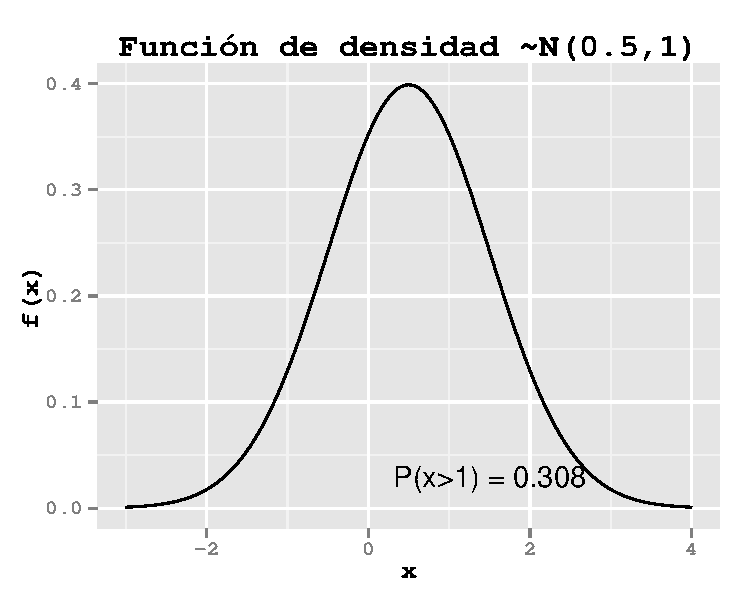
\includegraphics[width=\maxwidth]{figure/unnamed-chunk-3} 

}



\end{knitrout}

\newpage
\textbf{Problema 2}
Se utilizan dos máquinas para llenar botellas de plástico con un volumen neto de 16 onzas. El proceso de llenado se puede suponer normal. Los ingenieros del departamento de calidad sospechan que las dos máquinas llenan a diferente volumen, por lo que se realizó un experimento tomando una muestra al azar de 10 botellas llenadas por cada una de las dos máquinas.

\begin{table}[h!]
\centering
\begin{tabular}[t]{|c|c|c|c|}
\hline
\multicolumn{2}{|c|}{\textbf{máquina 1}}&\multicolumn{2}{|c|}{\textbf{máquina 2}}\\
\hline
16.03&16.01&16.02&16.03\\
16.04&15.96&15.97&16.04\\
16.05&15.98&15.96&16.02\\
16.05&16.02&16.01&16.01\\
16.02&15.99&15.99&16.00\\
\hline
\end{tabular}
\end{table}

\begin{enumerate}[a)]
  \item Pruebe la hipótesis de que el promedio de llenado de las dos máquinas es el mismo vs. es diferente.  Use $\alpha=0.05$. Primero suponiendo que las varianzas son homogéneas y después suponiendo que no son homogéneas.
  \item Calcule un intervalo del 95\% de confianza para la diferencia de las  medias de volumen de llenado de las máquinas.
\end{enumerate}

\noindent Veamos un boxplot de los datos por máquina:

\begin{knitrout}
\definecolor{shadecolor}{rgb}{0.969, 0.969, 0.969}\color{fgcolor}

{\centering 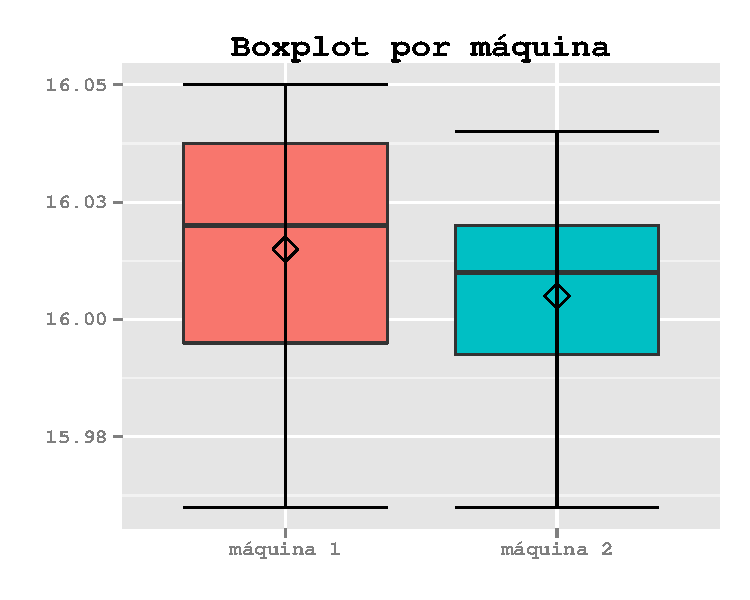
\includegraphics[width=\maxwidth]{figure/unnamed-chunk-4} 

}



\end{knitrout}

\begin{knitrout}
\definecolor{shadecolor}{rgb}{0.969, 0.969, 0.969}\color{fgcolor}\begin{kframe}
\begin{alltt}
\hlcom{# Pruebe la hipótesis de que el promedio de llenado de las dos máquinas }
\hlcom{# es el mismo vs. es diferente}
\hlcom{# Bajo el supuesto de varianzas iguales:}
\hlcom{# Método largo}
\hlcom{# Manipulamos los datos para los cálculos}
\hlstd{datos} \hlkwb{<-} \hlkwd{data.frame}\hlstd{(}\hlkwc{maquina1}\hlstd{=}\hlkwd{subset}\hlstd{(datos, trat} \hlopt{==} \hlstr{"máquina 1"}\hlstd{)[,} \hlstr{"vol"}\hlstd{],}
                    \hlkwc{maquina2}\hlstd{=}\hlkwd{subset}\hlstd{(datos, trat} \hlopt{==} \hlstr{"máquina 2"}\hlstd{)[,} \hlstr{"vol"}\hlstd{])}
\hlcom{# Cálculo de las medias}
\hlkwd{colMeans}\hlstd{(datos)}
\end{alltt}
\begin{verbatim}
## maquina1 maquina2 
##    16.02    16.00
\end{verbatim}
\begin{alltt}
\hlcom{# Cálculo de la diferencia de medias}
\hlstd{dif} \hlkwb{<-} \hlkwd{as.numeric}\hlstd{(}\hlkwd{colMeans}\hlstd{(datos)[}\hlnum{1}\hlstd{]} \hlopt{-} \hlkwd{colMeans}\hlstd{(datos)[}\hlnum{2}\hlstd{])}
\hlstd{S2_1} \hlkwb{<-} \hlkwd{var}\hlstd{(datos[,} \hlnum{1}\hlstd{])}
\hlstd{S2_2} \hlkwb{<-} \hlkwd{var}\hlstd{(datos[,} \hlnum{2}\hlstd{])}
\hlstd{S2_p} \hlkwb{<-} \hlstd{((n1} \hlopt{-} \hlnum{1}\hlstd{)} \hlopt{*} \hlstd{S2_1} \hlopt{+} \hlstd{(n2} \hlopt{-} \hlnum{1}\hlstd{)} \hlopt{*} \hlstd{S2_2)} \hlopt{/} \hlstd{(n1} \hlopt{+} \hlstd{n2} \hlopt{-} \hlnum{2}\hlstd{)}

\hlstd{t_0} \hlkwb{<-} \hlstd{dif}\hlopt{/}\hlstd{(}\hlkwd{sqrt}\hlstd{(S2_p}\hlopt{*}\hlstd{(}\hlnum{1}\hlopt{/}\hlstd{n1} \hlopt{+} \hlnum{1}\hlopt{/}\hlstd{n2))); t_0}
\end{alltt}
\begin{verbatim}
## [1] 0.7989
\end{verbatim}
\begin{alltt}
\hlcom{# Región de rechazo}
\hlstd{alpha} \hlkwb{<-} \hlnum{0.05}
\hlstd{gl} \hlkwb{<-} \hlstd{n1} \hlopt{+} \hlstd{n2} \hlopt{-} \hlnum{2}
\hlstd{t} \hlkwb{<-} \hlkwd{qt}\hlstd{(}\hlnum{1} \hlopt{-} \hlstd{(alpha}\hlopt{/}\hlnum{2}\hlstd{), gl)}
\hlcom{# P-value de 2 colas}
\hlkwd{pt}\hlstd{(t_0, gl,} \hlkwc{lower.tail} \hlstd{=} \hlnum{FALSE}\hlstd{)} \hlopt{*} \hlnum{2}
\end{alltt}
\begin{verbatim}
## [1] 0.4347
\end{verbatim}
\begin{alltt}
\hlcom{# Método corto}
\hlkwd{t.test}\hlstd{(datos[,} \hlnum{1}\hlstd{], datos[,} \hlnum{2}\hlstd{])}
\end{alltt}
\begin{verbatim}
## 
## 	Welch Two Sample t-test
## 
## data:  datos[, 1] and datos[, 2]
## t = 0.7989, df = 17.49, p-value = 0.435
## alternative hypothesis: true difference in means is not equal to 0
## 95 percent confidence interval:
##  -0.01635  0.03635
## sample estimates:
## mean of x mean of y 
##     16.02     16.00
\end{verbatim}
\end{kframe}
\end{knitrout}

\noindent Por lo que bajo la hipótesis $H_0: \mu_1 = \mu_2 (t= 0.7989,p>0.05)$ y asumiendo varianzas iguales, no existe evidencia significativa para rechazar que el promedio del llenado de botellas de la máquina 1 y 2 son iguales. Ahora veamos el caso cuando no consideramos que las varianzas son homogéneas.

\newpage

\begin{knitrout}
\definecolor{shadecolor}{rgb}{0.969, 0.969, 0.969}\color{fgcolor}\begin{kframe}
\begin{alltt}
\hlcom{# Bajo el supuesto de varianzas diferentes:}
\hlcom{# Método largo}
\hlcom{# t welch}
\hlstd{tw} \hlkwb{<-} \hlstd{dif} \hlopt{/} \hlstd{(}\hlkwd{sqrt}\hlstd{(S2_1}\hlopt{/}\hlstd{n1} \hlopt{+} \hlstd{S2_2}\hlopt{/}\hlstd{n2)); tw}
\end{alltt}
\begin{verbatim}
## [1] 0.7989
\end{verbatim}
\begin{alltt}
\hlcom{#región de rechazo}
\hlstd{gl_tw} \hlkwb{<-} \hlstd{(S2_1}\hlopt{/}\hlstd{n1} \hlopt{+} \hlstd{S2_2}\hlopt{/}\hlstd{n2)}\hlopt{**}\hlnum{2} \hlopt{/} \hlstd{(((S2_1}\hlopt{/}\hlstd{n1)}\hlopt{**}\hlnum{2}\hlopt{/}\hlstd{(n1} \hlopt{-} \hlnum{1}\hlstd{))} \hlopt{+} \hlstd{((S2_2}\hlopt{/}\hlstd{n2)}\hlopt{**}\hlnum{2}\hlopt{/}\hlstd{(n2}\hlopt{-}\hlnum{1}\hlstd{)))}
\hlstd{t2} \hlkwb{<-} \hlkwd{qt}\hlstd{(}\hlnum{1}\hlopt{-}\hlstd{(alpha}\hlopt{/}\hlnum{2}\hlstd{), gl_tw); t2}
\end{alltt}
\begin{verbatim}
## [1] 2.105
\end{verbatim}
\begin{alltt}
\hlcom{# P-value}
\hlkwd{pt}\hlstd{(tw, gl_tw,} \hlkwc{lower.tail} \hlstd{=} \hlnum{FALSE}\hlstd{)} \hlopt{*} \hlnum{2}
\end{alltt}
\begin{verbatim}
## [1] 0.435
\end{verbatim}
\begin{alltt}
\hlcom{# Método Corto}
\hlkwd{t.test}\hlstd{(datos[,} \hlnum{1}\hlstd{], datos[,} \hlnum{2}\hlstd{],} \hlkwc{var.equal}\hlstd{=F)}
\end{alltt}
\begin{verbatim}
## 
## 	Welch Two Sample t-test
## 
## data:  datos[, 1] and datos[, 2]
## t = 0.7989, df = 17.49, p-value = 0.435
## alternative hypothesis: true difference in means is not equal to 0
## 95 percent confidence interval:
##  -0.01635  0.03635
## sample estimates:
## mean of x mean of y 
##     16.02     16.00
\end{verbatim}
\end{kframe}
\end{knitrout}

\noindent Por lo qué observamos que tampoco existe evidencia para rechazar la hipótesis nula ($H_0: \mu_1 = \mu_2 (t= 0.7989,p>0.05)$), asumiendo que se tienen varianzas distintas. A continuación mostramos la prueba F para evaluar la exitencia de homocedasticidad

\begin{knitrout}
\definecolor{shadecolor}{rgb}{0.969, 0.969, 0.969}\color{fgcolor}\begin{kframe}
\begin{alltt}
\hlkwd{var.test}\hlstd{(datos[,} \hlnum{1}\hlstd{], datos[,} \hlnum{2}\hlstd{])}
\end{alltt}
\begin{verbatim}
## 
## 	F test to compare two variances
## 
## data:  datos[, 1] and datos[, 2]
## F = 1.41, num df = 9, denom df = 9, p-value = 0.6168
## alternative hypothesis: true ratio of variances is not equal to 1
## 95 percent confidence interval:
##  0.3503 5.6777
## sample estimates:
## ratio of variances 
##               1.41
\end{verbatim}
\end{kframe}
\end{knitrout}

\noindent Por lo que no hay evidencia para rechazar la hipótesis de homocedasticidad a un nivel de significancia del $0.05$.\\

\noindent Ahora calculamos los intervalos del $95\%$ de confianza para la diferencia de medias:

\begin{knitrout}
\definecolor{shadecolor}{rgb}{0.969, 0.969, 0.969}\color{fgcolor}\begin{kframe}
\begin{alltt}
\hlcom{# Bajo el supuesto de homocedasticidad}
\hlstd{ic_vi} \hlkwb{<-} \hlkwd{cbind}\hlstd{(dif} \hlopt{-} \hlstd{t} \hlopt{*} \hlkwd{sqrt}\hlstd{(S2_p}\hlopt{*}\hlstd{(}\hlnum{1}\hlopt{/}\hlstd{n1} \hlopt{+} \hlnum{1}\hlopt{/}\hlstd{n2)),}
               \hlstd{dif} \hlopt{+} \hlstd{t} \hlopt{*} \hlkwd{sqrt}\hlstd{(S2_p}\hlopt{*}\hlstd{(}\hlnum{1}\hlopt{/}\hlstd{n1} \hlopt{+} \hlnum{1}\hlopt{/}\hlstd{n2)))}
\hlkwd{colnames}\hlstd{(ic_vi)} \hlkwb{<-} \hlkwd{cbind}\hlstd{(}\hlstr{"límite inferior"}\hlstd{,}\hlstr{"límite superior"}\hlstd{);ic_vi}
\end{alltt}
\begin{verbatim}
##      límite inferior límite superior
## [1,]         -0.0163          0.0363
\end{verbatim}
\begin{alltt}
\hlcom{# Amplitud del intervalo}
\hlkwd{diff}\hlstd{(}\hlkwd{as.vector}\hlstd{(ic_vi))}
\end{alltt}
\begin{verbatim}
## [1] 0.05259
\end{verbatim}
\begin{alltt}
\hlcom{# Bajo el supuesto de no homocedasticidad}
\hlstd{ic_vd} \hlkwb{<-} \hlkwd{cbind}\hlstd{(dif} \hlopt{-} \hlstd{t2} \hlopt{*} \hlkwd{sqrt}\hlstd{(S2_1}\hlopt{/}\hlstd{n1} \hlopt{+} \hlstd{S2_2}\hlopt{/}\hlstd{n2),}
               \hlstd{dif} \hlopt{+} \hlstd{t2} \hlopt{*} \hlkwd{sqrt}\hlstd{(S2_1}\hlopt{/}\hlstd{n1} \hlopt{+} \hlstd{S2_2}\hlopt{/}\hlstd{n2))}
\hlkwd{colnames}\hlstd{(ic_vd)} \hlkwb{<-} \hlkwd{cbind}\hlstd{(}\hlstr{"límite inferior"}\hlstd{,}\hlstr{"límite superior"}\hlstd{);ic_vd}
\end{alltt}
\begin{verbatim}
##      límite inferior límite superior
## [1,]        -0.01635         0.03635
\end{verbatim}
\begin{alltt}
\hlcom{# Amplitud del intervalo}
\hlkwd{diff}\hlstd{(}\hlkwd{as.vector}\hlstd{(ic_vd))}
\end{alltt}
\begin{verbatim}
## [1] 0.0527
\end{verbatim}
\end{kframe}
\end{knitrout}

\noindent Por lo anterior vemos que el intervalo bajo el supuesto de homocedasticidad es más pequeño, además ambos intervalos contienen al cero, por lo que tenemos una confianza del $95\%$ de que no existe diferencia en el promedio de llenado de botellas en ambas máquinas. Es importante también mencionar que uno de los puestos que se usó al realizar los contrastes de hipótesis fue el de normalidad de los datos, por lo qué se debería aplicar una prueba para evaluar este supuesto.

\newpage
\textbf{Problema 3}
Considere un diseño de experimento unifactorial (efectos fijos) de 4 tratamientos donde se tienen un total de 24 unidades experimentales y conteste lo siguiente:

\begin{itemize}
  \item Complete la siguiente tabla ANOVA:
\end{itemize}

\begin{table}[h]
\centering
\begin{adjustbox}{max width=\textwidth}
\begin{tabular}{|l|c|ccc}
\hline
\rowcolor[HTML]{C0C0C0} 
\textbf{FV} & \multicolumn{1}{l|}{\cellcolor[HTML]{C0C0C0}\textbf{g.l.}} & \multicolumn{1}{l|}{\cellcolor[HTML]{C0C0C0}\textbf{S.C.}} & \multicolumn{1}{l|}{\cellcolor[HTML]{C0C0C0}\textbf{C.M.}} & \multicolumn{1}{l|}{\cellcolor[HTML]{C0C0C0}\textbf{F}} \\ \hline
\cellcolor[HTML]{C0C0C0}\textbf{Modelo} &  & \multicolumn{1}{c|}{} & \multicolumn{1}{c|}{} & \multicolumn{1}{c|}{0.5655} \\ \hline
\cellcolor[HTML]{C0C0C0}\textbf{Error} &  & \multicolumn{1}{c|}{} & \multicolumn{1}{c|}{16.02} &  \\ \cline{1-4}
\cellcolor[HTML]{C0C0C0}\textbf{Total} &  &  &  &  \\ \cline{1-2}
\end{tabular}
\end{adjustbox}
\end{table}

\noindent La tabla la podemos completar de la siguiente forma:\\

\begin{table}[h]
\centering
\begin{adjustbox}{max width=\textwidth}
\begin{tabular}{|l|c|c|cc}
\hline
\rowcolor[HTML]{C0C0C0} 
\textbf{FV} & \textbf{g.l.} & \textbf{S.C.} & \multicolumn{1}{c|}{\cellcolor[HTML]{C0C0C0}\textbf{C.M.}} & \multicolumn{1}{c|}{\cellcolor[HTML]{C0C0C0}\textbf{F}} \\ \hline
\cellcolor[HTML]{C0C0C0}\textbf{Modelo} & t - 1 = 4 - 1 = 3 & SSt = CMt * (t - 1) = 27.178 & \multicolumn{1}{c|}{CMt = F * CME = 9.059} & \multicolumn{1}{c|}{F = CMt / CME = 0.5655} \\ \hline
\cellcolor[HTML]{C0C0C0}\textbf{Error} & n - t = 96 - 4 = 92 & SSE = CME * (n - t) = 16.02 * 92 = 1473.84 & \multicolumn{1}{c|}{CME = 16.02} &  \\ \cline{1-4}
\cellcolor[HTML]{C0C0C0}\textbf{Total} & n - 1 = 96 -1 = 95 & SStotal = SSt + SSE &  &  \\ \cline{1-3}
\end{tabular}
\end{adjustbox}
\end{table}

\begin{itemize}
  \item Determine el valor $\hat{\sigma^2}$
\end{itemize}
De la tabla sabemos que $CME = \hat{\sigma^2} = 16.02$

\begin{itemize}
  \item Con $\alpha = 0.05$ se rechaza o no la hipótesis de igualdad de medias?
\end{itemize}
\begin{knitrout}
\definecolor{shadecolor}{rgb}{0.969, 0.969, 0.969}\color{fgcolor}\begin{kframe}
\begin{alltt}
\hlstd{alpha} \hlkwb{<-} \hlnum{0.05}
\hlkwd{qf}\hlstd{(}\hlnum{1} \hlopt{-} \hlstd{alpha,} \hlkwc{df1}\hlstd{=} \hlnum{3}\hlstd{,} \hlkwc{df2} \hlstd{=} \hlnum{92}\hlstd{)}
\end{alltt}
\begin{verbatim}
## [1] 2.704
\end{verbatim}
\end{kframe}
\end{knitrout}
Entonces sabemo que valores grandes de $F$ llevan a rechazar la hipótesis de nula de igualdad de medias, pero como $F = 0.5655 < F_{t-1, n-t}^{0.05} = 2.704)$ no tenemos evidencia para rechzar la hipótesis nula a una significancia del $5\%$.


\begin{itemize}
  \item Con $\alpha = 0.01$ se rechaza o no la hipótesis de igualdad de medias?
\end{itemize}
\begin{knitrout}
\definecolor{shadecolor}{rgb}{0.969, 0.969, 0.969}\color{fgcolor}\begin{kframe}
\begin{alltt}
\hlstd{alpha} \hlkwb{<-} \hlnum{0.01}
\hlkwd{qf}\hlstd{(}\hlnum{1} \hlopt{-} \hlstd{alpha,} \hlkwc{df1}\hlstd{=} \hlnum{3}\hlstd{,} \hlkwc{df2} \hlstd{=} \hlnum{92}\hlstd{)}
\end{alltt}
\begin{verbatim}
## [1] 4.002
\end{verbatim}
\end{kframe}
\end{knitrout}
En este caso $F = 0.5655 < F_{t-1, n-t}^{0.05} = 4.002)$ por lo que tampoco tenemos evidencia para rechazar la hipótesis nula a una significancia del $5\%$.




\end{document}
